
%(BEGIN_QUESTION)
% Copyright 2006, Tony R. Kuphaldt, released under the Creative Commons Attribution License (v 1.0)
% This means you may do almost anything with this work of mine, so long as you give me proper credit

Shown here is a schematic diagram for a simple, analog electronic, proportional-only controller:

$$\includegraphics[width=15.5cm]{i01534x01.eps}$$

Explain what you would have to do to increase the proportional band of this controller circuit, and also determine whether it is {\it direct-acting} or {\it reverse-acting}.

\vskip 10pt

Now, consider this modification to the controller circuit, giving it {\it proportional} and {\it derivative} control capability, sometimes referred to as P+D or PD control:

$$\includegraphics[width=15.5cm]{i01534x02.eps}$$

Explain how the additional module (Module 6) implements derivative control action, and what would have to be changed in the circuit to increase $\tau_d$ (i.e. make the derivative action more aggressive).

\underbar{file i01534}
%(END_QUESTION)





%(BEGIN_ANSWER)

To increase proportional band (reduce the gain), move the potentiometer wiper to the right (Module 4).  This is a {\it reverse-acting} controller.

\vskip 10pt

To increase the aggressiveness of derivative action, increase the capacitor value (Module 6) and/or decrease the summing input resistor value in Module 5 that accepts Module 6's output signal.

%(END_ANSWER)





%(BEGIN_NOTES)

To increase the aggressiveness of derivative action, increase the capacitor value (Module 6) and/or decrease the summing input resistor value in Module 5 that accepts Module 6's output signal.

%INDEX% Control, derivative: analog electronic controller

%(END_NOTES)


